\documentclass[letter, 10pt]{article}
\usepackage[spanish]{babel}
\usepackage[utf8]{inputenc}
\usepackage{amsfonts}
\usepackage{amsmath}
\usepackage{graphicx}
\usepackage{url}
\usepackage[top=3cm,bottom=3cm,left=3.5cm,right=3.5cm,footskip=1.5cm,headheight=1.5cm,headsep=.5cm,textheight=3cm]{geometry}


\begin{document}
\title{Inteligencia Artificial \\ \begin{Large}Estado del Arte: Manejo de Trenes en Estaciones Ferroviarias\end{Large}}
\author{Martín Villanueva A.}
\date{23 de Mayo de 2016}
\maketitle


%--------------------No borrar esta secci\'on--------------------------------%
\section*{Evaluación}

\begin{tabular}{ll}
Resumen (5\%): & \underline{\hspace{2cm}} \\
Introducción (5\%):  & \underline{\hspace{2cm}} \\
Definición del Problema (10\%):  & \underline{\hspace{2cm}} \\
Estado del Arte (35\%):  & \underline{\hspace{2cm}} \\
Modelo Matemático (20\%): &  \underline{\hspace{2cm}}\\
Conclusiones (20\%): &  \underline{\hspace{2cm}}\\
Bibliografía (5\%): & \underline{\hspace{2cm}}\\
 &  \\
\textbf{Nota Final (100\%)}:   & \underline{\hspace{2cm}}
\end{tabular}
%---------------------------------------------------------------------------%
\vspace{2cm}


\begin{abstract}

\end{abstract}

\section{Introducción} \label{intro}


\section{Definición del Problema} \label{probdef}
La definición del problema que se expone en esta sección, esta basada en \textit{ROADEF/Euro Challenge 2014} 
\cite{Problem}, con ciertas modificaciones y simplificaciones que se detallan en lo que sigue.


Como se mencionó anteriormente, el principal propósito del problema, consiste en encontrar la mejor
manera de manejar trenes en estaciones ferroviarias, entre las llegadas, las salidas y el uso de recursos
que hacen en la estación. Todo este proceso puede ser visto como una secuencia de subproblemas, sin embargo
aquí se trata y modela de una manera integrada. En vista de que el problema tiene en cuenta una gran 
cantidad de \textit{dimensiones}, a continuación se describen cada una de ellas de manera simple.

\begin{description}
	\item[\textsc{Horizonte de Planificación.}] 
	El horizonte de planificación corresponde al conjunto de instantes de tiempo (\textit{discretizados}),
	sobre el que se espera realizar toda la planificación del sistema. El formato de cada instante de tiempo
	es $(\text{d hh:mm:ss})$, con $\text{d } \in \{1, nbDays\}$ el día respectivo, $\text{hh } \in \{0,23\}$ 
	la hora, $\text{mm } \in \{0,59\}$ el minuto, y $\text{ss } \in \{0,59\}$ el segundo. El conjunto de todos
	los intantes se denominará $\mathcal{H}$. Con esta representación, el menor intervalo de tiempo permitido
	es un segundo, lo que permite representar el tiempo con una alta precisión. Sin embargo dependiendo de la 
	instancia, pueden tomarse duraciones más largas (múltiplos de segundos, o minutos), reduciendo el tamaño del
	\textit{espacio de búsqueda}.

	\item[\textsc{Llegadas.}]
	Las llegadas corresponden al ingreso de trenes en el sistema. Los tiempos de llegada (a la plataforma),
	son datos de entrada y por lo tanto no modificables. Hay que tomar en cuenta que los trenes entran al
	sistema/estación un tiempo antes que su hora de llegada. Durante este periodo intermedio realizan una
	\textit{secuencia de llegada}, que representan la secuencia de recursos (y los respectivos tiempos) de 
	los cuales hace uso el tren, antes de llegar a la plataforma para que los pasajeros bajen. Los aspectos
	y restricciones a considerar son los siguientes:
	\begin{enumerate}
		\item Cada llegada $a \in \mathcal{A}$ tiene un conjunto de plataformas preferidas a usar $\text{prefPlat}_a$.
		 Esta es una reestricción blanda, pero penalizada en la función objetivo.
		\item Existen tiempos ideal y máximo de permanencia en la plataforma: $\text{idealDwell}_a$ y $\text{maxDwell}_a$.
		Tiempos inferiores y superiores al $\text{idealDwell}_a$ son penalizados, pues el primero disminuye la satisfacción
		de los pasajeros que deben bajar, y el segundo constituye un mal uso de los recursos del sistema. En cualquier caso,
		el tiempo de permanencia no puede superar el máximo $\text{maxDwell}_a$.
		\item Es posible no cubrir una llegada, esto es, que el tren asociado a la llegada no entre a la estación. Como es de esperar, esto incurre una penalización.
	\end{enumerate}

	\item[\textsc{Salidas.}]
	Las salidas corresponden a la ida de trenes del sistema. Análogo a las entradas, los tiempos y secuencias de
	salida (ruteo entre los recursos hasta salir de la estación) son datos de entrada fijos. La principal tarea a
	cumplir aquí, es asignar un tren a cada salida. Los aspectos y restricciones a considerar son los siguientes:
	\begin{enumerate}
		\item No asignar un tren a un salida es penzalizado gravemente en la función objetivo. Adicionalmente, no
		puede asignarse más de un tren a un salida.
		\item Cada salida $d \in \mathcal{D}$ tiene un conjunto de plataformas preferidas a usar $\text{prefPlat}_d$.
		Esta es un reestricción blanda, pero penalizada en la función objetivo.
		\item Existen tiempos ideal y máximo de permanencia en la plataforma: $\text{idealDwell}_d$ y $\text{maxDwell}_d$.
		Las penalizaciones siguen la misma lógica que en las llegadas.
		\item Una salida tiene asociado un conjunto de categorías de trenes compatibles $\text{compCatDep}_d$. Esto va asociado a las características que debe tener el tren para hacer el viaje, y constituye una reestricción fuerte
		(no se puede violar).
		\item Cada tren tiene una \textit{distancia por recorrer antes de manteción} ($\text{remDBM}$) y \textit{tiempo de viaje antes de mantención} ($\text{remTBM}$). Cada salida tiene asociada un distancia y tiempo necesario para realizar el viaje. Luego el tren asignado debe tener $\text{remDBM}$ y $\text{remTBM}$ mayor o iguales a los que requiere la salida.

	\end{enumerate}

	\item[\textsc{Trenes.}]
	Un tren se define como una unidad movil de \textit{visita} en el sistema. Esto quiere decir que no se considera como tren
	a la unidad física; un mismo tren que visita más de una vez el sistema, se toma como trenes distintos. El conjunto de trenes $\mathcal{T}$ se compone de dos tipos de trenes: Los trenes presentes en la estación desde el inicio del horizonte de tiempo $\mathcal{T}_I$,  y los trenes asociados a llegadas $\mathcal{T}_A$.
	Las principales consideraciones a tener con los trenes son las siguientes:
	\begin{enumerate}
		\item Cada tren es una unidad atómica; No se pueden separar en vagones, ni recombinarlos con los de otros trenes. Por lo tanto un tren es la unidad de asignación más pequeñas. Como nota, esta reestricción es acorde a la naturaleza de los trenes modernos.
		\item Un tren $t \in \mathcal{T}$ esta asociado a una categoría $\text{cat}_t$, que define las características técnicas que comparten. Se puede pensar en los trenes de una misma categoría como el mismo tren (fabricado en serie por alguna compañia), pero con diferentes condiciones de mantención iniciales. 
		\item No ocupar los trenes inicialmente en el sistema es una opción posible, pero será penalizada. Tales trenes no usarán recursos durante el horizonte de planificación.
		\item Asociado una llegada y salida, puede haber un \textit{reuso}. Esto consiste en definir previamente (dato de entrada) cual tren que viene llegando, será asignado a una salida. Existe un costo asociado a no cumplir un reuso dado. Los reusos no serán respetados, siempre y caundo esto beneficie en mayor medida a otros objetivos. Por último,
		cada salida $d \in \mathcal{D}$ puede estar asociada a lo más en un reuso con la entrada $a \in \mathcal{A}$, y de igual modo al revés.
	\end{enumerate}

	\item[\textsc{Mantenciones.}]
	Los trenes deben ser sometidos a mantenciones regularmente, de modo que cumplan las condiciones de seguridad y comodidad necesarias que requiere cada salida. Cómo se mencionó anteriormente, hay dos parámetros a considerar en las manteciones:
	\begin{enumerate}
		\item \textbf{TBM}, el tiempo de viaje antes de realizar mantención (\textit{Time Before Maintanance}). Este va asociado al comodidad de los pasajeros (que el tren este limpio, asientos en buenas condiciones, etc).
		\item \textbf{DBM}, la distancia de viaje antes de realizar mantención (\textit{Distance Before Maintanance}). Se 
		relaciona con condiciones de seguridad (combustible, estado de frenos, etc).  
	\end{enumerate}
	Las operaciones de mantención básicamente reajustan los valores $\text{remTBM}$ y $\text{remDBM}$ a los valores máximos de cada tren. Las consideraciones a tener en cuenta son:
	\begin{enumerate}
		\item El movimiento de un tren dentro de la estación de resta a $\text{remTBM}$ y $\text{remDBM}$ (despreciables en comparación al de los viajes).
		\item Las mantenciones se realizan en las \textit{Instalaciones de Mantenimiento} descritas en la siguiente sección. 
	\end{enumerate}

	\item[\textsc{Recursos de Infraestructura.}]
	Los trenes en el sistema, estan siempre haciendo uso de algun recurso (ya sea moviendose o estacionados). Estos recursos
	son $5$ tipos: pistas simples $\mathcal{S}$, plataformas de llegada o salida $\mathcal{P}$, instalaciones de mantenimiento $\mathcal{F}$, grupos de pistas $\mathcal{K}$ y estacionamientos $\mathcal{Y}$. Las pistas simples, plataformas, y instalaciones de mantenimiento son consideradas como porciones individuales de una pista. Por otro lado 
	los grupos de pistas se constituyen de varias pistas de forma agregada. Una configuración típica para los recursos del
	sistema pueden verse en Figura \ref{fig:resources}.
 	\begin{figure}[htpb!]
	\centering
	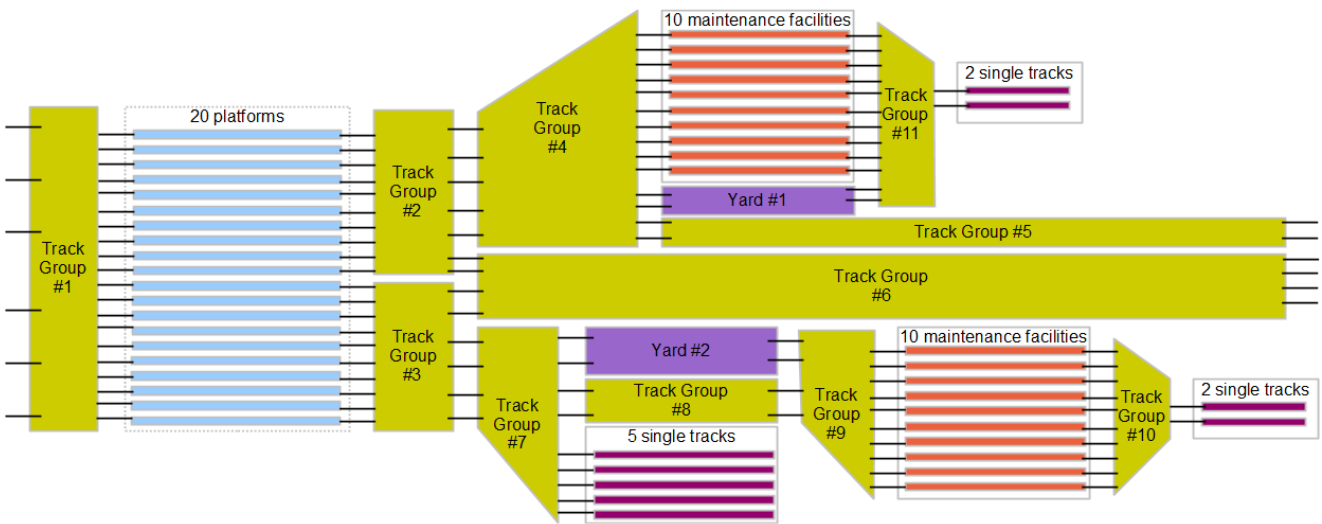
\includegraphics[width=12cm]{resources}
	\caption{Ejemplo de recursos de infraestructura (Fuente \cite{Problem})}
	\label{fig:resources}
	\end{figure}

	Es muy imporatente considerar la forma en que los trenes se mueven entre los recursos y sus restricciones. Los principales aspectos se listan como sigue:
	\begin{enumerate}
		\item Un mismo tren no puede estar ocupando dos recursos en el mismo instante de tiempo (algo que sí sucede en la realidad). Por lo tanto cada tren se considera como un objeto puntal que puede moverse de un recurso a otro de modo instantaneo.
		\item Cada recurso $r \in \mathcal{R}$ tiene un conjunto de recursos vecinos $\text{neighSet}_r$, que definen las posibles transiciones de un tren, esto es, un tren en un recurso $r$, sólo puede moverse a un recurso vecino en $\text{neighSet}_r$.
		\item Usualmente (hay excepciones) cada recurso puede ser accedido por dos lados, que se denotan A y B. Entonces el conjunto de recursos vecinos de $r$ puede ser descompuesto en $\text{neighSet}_r = \text{neighSet}_r^A \cup \text{neighSet}_r^B$. Adicionalmente se tiene como reestricción $\text{neighSet}_r^A \cap \text{neighSet}_r^B = \emptyset$, esto es, que no se generen ciclos entre los recursos.
		\item Las excepciones al punto anterior las constituyen los recursos al extremo del sistema, por donde los trenes entran o salen.
		\item Los recursos tienen en ambos extremos \textit{puertas} por donde se realiza la transición hacia otro recurso.
		Cada puerta $g \in \mathcal{G}_r$ de un recurso $r$, esta asociada a una única puerta de un recurso vecino (si la puerta esta en el fin del sistema, puede no tener puerta vecina asociada).
		\item Las pistas simples, plataformas y instalaciones de mantención tienen como máximo una puerta en cada lado.
		\item Los grupos de pistas y estacionamientos pueden tener mas de una puerta en cada lado. 
		\item Algunos recursos pueden ser utilizados sólo por un tipo específico de tren (por lo general en las estaciones de mantenimiento). Por ello cada recurso $r$ tiene su conjunto de categorías de trenes compatibles $\text{compCatRes}_r$.
		\item Pueden haber recursos ocupados con antelación en el sistema. Estos factores son externos al problema y fijos, siendo algunos ejemplos: trenes de mantenimiento, trenes que no terminan en la estación, trenes externos de otras compañias, entre otros. 
	\end{enumerate}

	Teniendo una idea de la mecánica de uso de recursos del sistema, a continuación se entregan detalles específicos de cada tipo de recurso.
	\begin{enumerate}
		\item \textbf{Pistas Simples.} Corresponden a pistas unitarias, usada para el movimiento de los trenes dentro de la estación. Estos son (usualmente) los recursos que utilizan los trenes para entrar y salir del sistema. Cada pista simple $s \in \mathcal{S}$ tiene asociado un largo total $\text{lenght}_s$ y cantidad de trenes $\text{capa}_s$,
		que debe ser respetado en cada instante de tiempo.
		\item \textbf{Plataformas.} Estas representan las pistas en donde los pasajeros pueden salir o abordar un tren. Por lo tanto son estas, las que deben ser asignadas a cada llegada o salida respectivo. A diferencia de las pistas simples, una plataforma $p \in \mathcal{P}$ sólo esta restrigida en capacidad por su largo $\text{lenght}_p$.
		\item \textbf{Instalaciones de Mantenimiento.} Estas instalaciones son pistas donde los trenes se detienen a realizar su respectiva mantención (reajustar su TBM y DBM). Es muy importante notar que cada instalación de mantenimiento $f \in \mathcal{F}$ esta equipada para hacer sólo un tipo de operación (``D'' o ``T''). Por lo tanto si un tren requiere hacer ambos mantenimientos, deberá pasar por dos instalaciones distintas. Por último, al igual que las plataformas, su capacidad esta restringida por su largo $\text{lenght}_f$.
		\item \textbf{Grupos de Pistas.} Son un conjunto agregado de pistas, utilizados para mover a los trenes entre los distintos recursos del sistema. Todas las puertas de un lado son alcanzables desde el otro (y viceversa), por lo tanto si en un lado hay $m$ puertas y en el otro lado hay $n$, existen $m\ n$ posibles rutas para atravesar el grupo de pistas. Un grupo de pistas $k \in \mathcal{K}$ tiene dos parámetros importantes: el tiempo necesario para atravesar $k$ $\text{trTime}_k$ (constante), y el tiempo mínimo que debe haber entre dos trenes sucesivos para que no esten tan cerca $\text{hwTime}_k$. Técnicamente los grupos de pistas son una estructura compleja, que debe manejar normas de seguridad y conflictos que suelen ocurrir. Sin embargo el problema se abstrae de esta complejidad, viendo a tal estructura como una \textit{caja negra}. 
		\item \textbf{Estacionamientos.} Al igual que el anterior, son también un conjunto de pistas pero utilizadas para estacionar trenes. Por lo tanto un tren puede permanecer en un estacionamiento sin limites de tiempo. Un estacionamiento $y \in \mathcal{Y}$ esta límitado en capacidad por la cantidad de trenes permitidos $\text{capa}_y$.
	\end{enumerate}


	\item[\textsc{Objetivo.}] Tal como se plantea el problema, la objetivo general se descompone en múltiples objetivos,
	que corresponden a minimizar las penalizaciones descritas anteriormente. Luego la función a minimizar es:
	\begin{align}
		f = f^{\text{uncov}} + f^{\text{over}} + f^{\text{plat}} + f^{\text{pref}} + f^{\text{reuse}},
		\label{eq:gobj}
	\end{align}
	donde cada una representa:
	\begin{enumerate}
		\item $f^{\text{uncov}}$: Costo por no cubrir una salida.
		\item $f^{\text{over}}$: Costo asociado al sobre-mantenimiento.
		\item $f^{\text{plat}}$: Costo por uso de las plataformas.
		\item $f^{\text{pref}}$: Costo por no respetar la preferencia de uso de plataforma.
		\item $f^{\text{reuse}}$: Costo por no respetar un reuso dado inicialmente. 
	\end{enumerate}
	un análisis más detallado de (\ref{eq:gobj}) será visto en la sección de Modelo Matemático.
	\item[\textsc{Solución Esperada.}] Como solución al problema, se espera una conjunto de programación de eventos
	para cada tren, esto es, una secuencia de eventos junto con los recursos usados, y los tiempos asociados. Los diferentes tipos de eventos pueden ser: \texttt{EnterSystem}, \texttt{ExitSystem}, \texttt{Arrival}, \texttt{Departure}, \texttt{EnterResource}, \texttt{ExitResource}, \texttt{BeginMaintenance} y \texttt{EndMaintenance}. Un ejemplo de posible solución para un tren dado se da en Figura \ref{fig:sched}.
	 \begin{figure}[htpb!]
	\centering
	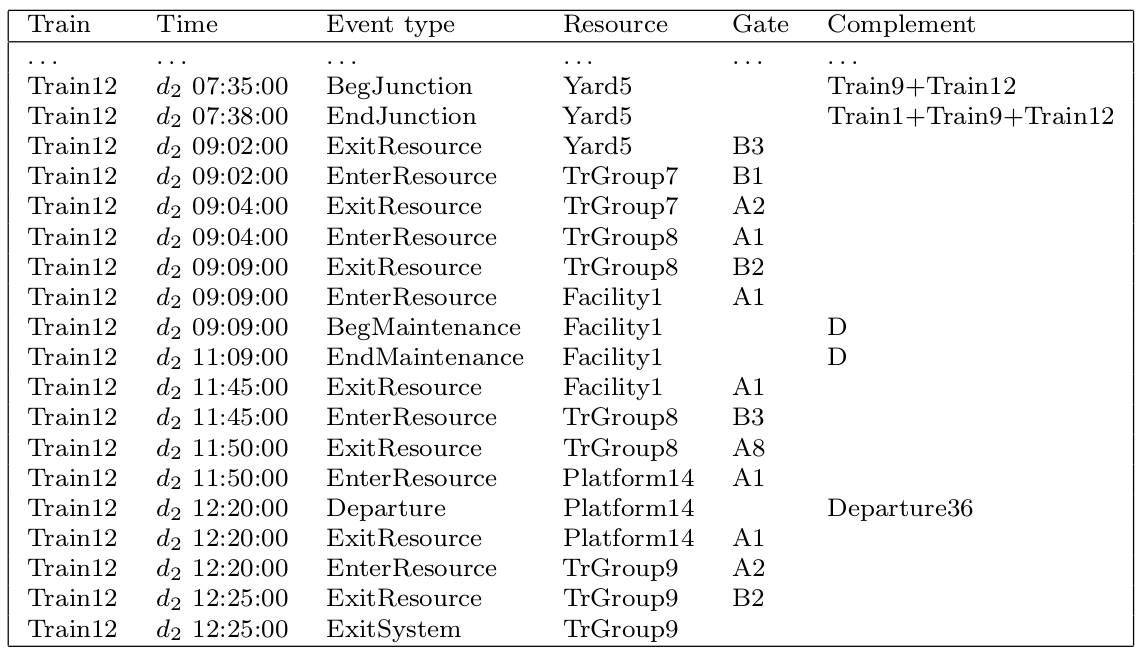
\includegraphics[width=12cm]{sched}
	\caption{Extracto de programación de eventos para un tren dado (Fuente \cite{Problem})}
	\label{fig:sched}
	\end{figure}
	Teniendo esta información para todos los trenes, sera posible inferir el estado del sistema y sus recursos, en cada instante del horizonte de planificación.

\end{description}




\section{Estado del Arte} \label{SoA}
En la presente sección se hace un estudio acerca de como nace este problema y la forma en que ha sido abordado. Pese a que  hay gran cantidad de trabajo realizado (y en desarrollo) al respecto \cite{RoadefResults}, hay pocos que han sido publicados. Por lo tanto también se expondrán las variantes o sub-problemas más conocidos, así como los disintitos enfoques con los que han sido abordados.

\begin{description}
	\item[\textsc{Inicios del Problema.}] En el problema de estudio en el presente artículo, corresponde a una versión \textit{simplificada} del problema propuesto en el ROADEF/EURO Challenge 2014 \cite{Problem}, competencia organizada
	por la \textit{SFrench Operational Research (OR) and Decision Support Society} (ROADEF) y la \textit{European Operational Research Society} (EURO) en conjunto con la \textit{Société Nationale des Chemins de Fer Français} (SNFC).
	El objetivo de esta, fue encontrar la mejor forma realizar el manejo, ruteo y asignación de trenes en una estación ferroviaria, tal como se explicó en la sección \ref{probdef}. La simplifación nombrada, consiste en que se da por alto una de las dimensiones del problema, que es la unión y separación de trenes. Como se explicó en la sección \ref{probdef},
	los trenes son las unidades de asignación más pequeñas a utilizar, esto es, no pueden ser separados ni recambinados sus vagones. Sin embargo, en la medida de poder satisfacer salidas con gran cantidad de pasajeros, es posible \textit{unir} 
	dos trenes en el sistema para cumplir con la capacidad. El proceso de \textit{unir} y \textit{separar} trenes en las estaciones es llevado en los \textit{grupos de pistas}, y agrega una complejidad considerable a la formulación y a su solución.
	Una buena cantidad de equipos lograron dar con soluciones satisfactorias \cite{RoadefResults}. Algunas de estas se detallan en lo que sigue.

	\item[\textsc{Propuestas de Solución.}]
	El primero trabajo publicado corresponde a \textit{A Math-Heuristic Framework for the ROADEF/EURO Challenge 2014} \cite{MathHeuristic}, cuyos autores participaron en la categoría junior del concurso obteniendo el segundo lugar. El nombre \textit{math-heuristic} se debe a que se combinan métodos exactos con heurísticas para hallar una solución. El problema original se aborda como cuatros sub-problemas, tal como se describe en la figura \ref{fig:diagram}. Cada etapa se resume a continuación:
	\begin{enumerate}
		\item \textsc{Arrival\&Departure Matching}. En esta primera etapa, se intenta hacer un \textit{match} para cada salida, con un tren compatible (tren inicial o de llegadas). El problema es planteado como MIP (\textit{Mixed Integer Programming}), con básicamente dos objetivos: Minimizar el número de cancelaciones de salidas (salidas sin cubrir) y maximizar la cantidad de reusos entre las llegadas y salidas. Debido a la gran cantidad de variables involucradas, este es resuelto usando el método de generación de columnas. Para generar los \textit{matches} se generan los conjuntos $\text{Comp}(d)$ y $\text{Comp}(t)$ que contienen los trenes compatibles para cada salida $d$ y las salidas compatibles a cada tren $t$, respectivamente. Estos se computan filtrando las combinaciones inviables, y utilizando heurísticas (eg. eliminando \textit{matches} en espacios de tiempo muy grandes). 
		\item \textsc{Platform Assignment}. En segundo lugar es necesario asignar las plataformas a utilizar por cada llegada y salida a cubrir. Se intenta aquí asignar de manera que se minimizen las cancelaciones de llegada y salidas, y que cada una sea asignada a su plataforma preferida, en la medida de lo posible. Este tambien se plantea como MIP, pero se resuelve buscando una solución exacta.
		\item \textsc{Arrival\&Departure Sequence Assigner}. Luego para cada una de las llegadas y salidas a cubrir, se generan patrones de uso de los grupos de pistas, de modo que no existan conflictos entre en las secuencias respectivas, ni el uso de recursos impuestos inicialmente. 
		\item \textsc{Simulated Annealing / Train Routing}. En última instancia, \textit{Simulated Annealing} (SA) es utilizado para generar rutas (secuencia de recursos) que los trenes realizan en la estación. Para ello en cada iteración se \textit{rutea} a un tren, seleccionando una ruta aleatorea basada en los \textit{matches} y asignación de recursos anteriores. Cada nueva solución es aceptada dependiendo del costo y temperatura.
	\end{enumerate}
	Cabe mencionar el este articulo no trabaja las condiciones de uniones de trenes en llegadas y salidas. En definita este enfoque se basa en ocupa SA para generar rutas aleatoreas, apoyandose en resultados precomputados para la utilización de recursos y evitar conflictos.
	\begin{figure}[htpb!]
	\centering
	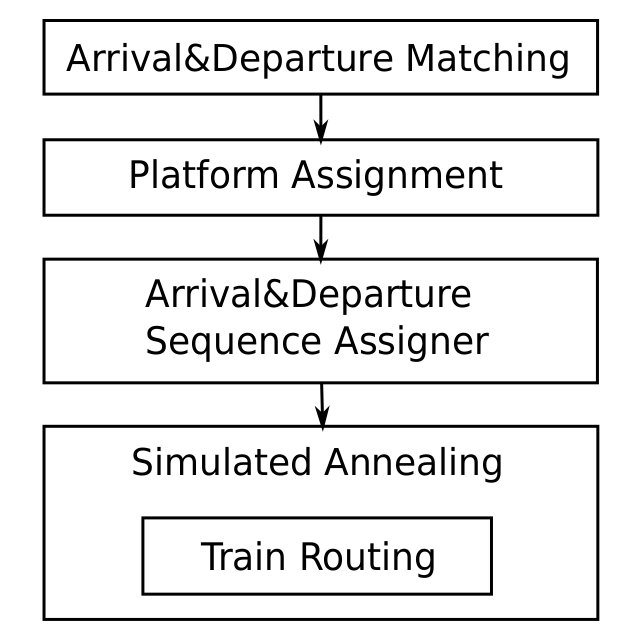
\includegraphics[width=4cm]{diagram}
	\caption{Esquema de solución en Math-Heuristic Framework (Fuente \cite{MathHeuristic})}
	\label{fig:diagram}
	\end{figure}

	El segundo trabajo \textit{Roadef Challenge 2014: A Modeling Approach, Rolling stock unit management on railway sites}\cite{ModelingApproach}, presenta un acabado estudio con un modelo similar al anterior; Descompone el problema original en dos estapas de decisión: asignación y enrutamiento. La idea de generar estos dos subproblemas, es reducir la complejidad inicial, y ocupar la técnica de resolución indicadda para cada uno. Por un lado, la primera etapa se compone básicamente de asignar trenes (de las llegadas o inicialmente en el sistema) a las salidas, asignar plataformas, y el resto de recursos del sistema. Este tipo de problemas son fácilmente formulables en MIP, y pueden ser resueltos de manera eficiente con dicha representación (por generación de columnas). Por otro lado, la fase de enrutamiento de trenes en la estación se desacopla totalmente de la fase de asignación, y se propone utilizar CP (\textit{Constraint Programming}) para su solución, pues es la opción más viable y eficiente. Algunos detalles se listan a continuación para cada fase (Ver Figura \ref{fig:diagram2}).
 	\begin{figure}[htpb!]
	\centering
	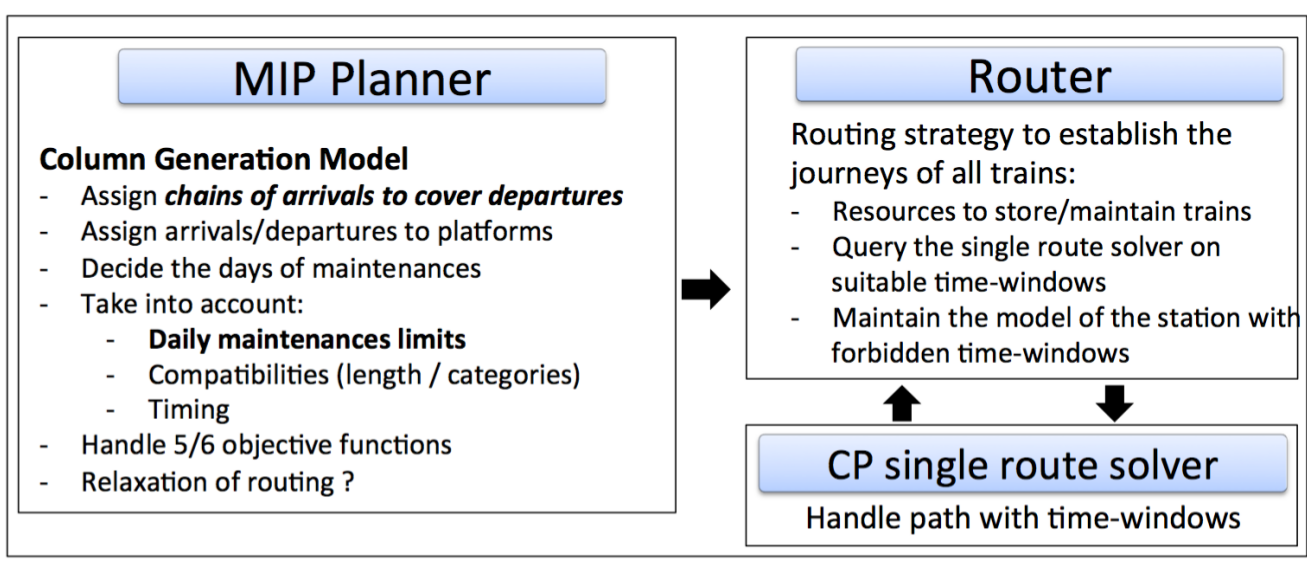
\includegraphics[width=8cm]{diagram2}
	\caption{Esquema de solución de Modeling Approach (Fuente \cite{ModelingApproach})}
	\label{fig:diagram2}
	\end{figure}

	\begin{enumerate}
		\item \textsc{Asignacion.} El problema de asignación abarca asignar trenes a las salidas, asignar plataformas a las llegadas y salidas y asignar las mantenciones. La función objetivo que se plantea planteada considera: \textit{llegadas/salidas no cubiertas}, \textit{trenes iniciales no usados}, \textit{plataformas preferidas no satisfechas}, \textit{reusos no satisfechos} y \textit{sobre manteciones}. Todo lo anterior se modela por medio de MIP. Se hace luego una extensión a esta formulación para considerar el caso de llegadas \textit{enlazadas} con salidas previas, verificando que tal problema se reduce a \textit{Dependent Matching Problem} (DPM) que es NP-completo.  
		\item \textsc{Enrutamiento.} Para esta se parte de la premisa de que es posible computar las rutas de los trenes en la estación, sin cuestionar los resultados previos de la fase de asignación. Aquí modela la estación y sus recursos como un grafo, y muestra que el problema de enrutar un sólo tren se reduce a \textit{Resource Constrained Shortest Path Problem} (RCSPP) que es NP-hard. En base a esto, un modelo de CP es inferido para definir las rutas, y luego se computan una por una las rutas de todas las llegadas/salidas, de modo que si el \textit{solver} de CP es incapáz de encontrar una solución, se cancela la llegada/salida asociada.
	\end{enumerate}
	Los autores reconocen que uno de los puntos debiles del modelo propuesto está en la estrategia de enrutamiento, sobre la cual es posible usar distintas heurísticas para tratar el problema de formas más integrada, y así minimizar las cancelaciones. 



	\item[\textsc{Problemas Relacionados.}] El problema en estudio ha sido estudiado y abordado múltiples maneras; Distintos objetivos, restricciones y métodologías de solución. En el presente estudio, se presentan las más notables entre estas.

	Uno de los prencipales sub-problemas es conocido como \textit{Train Timetabling Problem}, el cual consiste en generar una planificación horaria para los trenes en una estación, para cubrir las salidas satisfaciendo restricciones particulares del sistema. Este problema ha sido modelado y resuelto mediante múltiples técnicas. Uno de los primeros estudio formales lo entrega Caprara \cite{Caprara}, quien modela el problema y demuestra que es NP-hard, siendo una generalización del MSSP (\textit{Maximum Stable Set Problem}).

	Una solución al TTP en con una sola pista es propuesta por Cacchiani et al. \cite{Cacchiani}, basado en método de generación de columnas. Aquí se propone un modelo de ILP (\textit{Integer Linear Programming}) en donde cada variable, corresponde a la secuencia de programaciones horarias de un tren, denominadas \textit{path variables} (variables de ruta). Esto genera una gran cantidad de combinaciones y posibles soluciones, por lo tanto es adecuado de resolver con técnicas generación de columnas. Adicionalmente un método básado en heurísticas y \textit{local search} es propuesto e implementado. Ambas propuestas fueron probadas con instancias reales de \textit{Rete Ferroviaria Italian} (RFI). Los resultados mostraron que pese a que el número de variables de la primera formulación crece exponencialmente, estos son resueltos en tiempos razonables. Por otro el modelobasado en heurísticas entrega mejores resultados, sin embargo los tiempos de computación son considerablemente mayores.

	Una variante interesante propone Mohammad et al. \cite{Mohammad} en la resolución del TTP con una sola vía. Se formula el modelo como MIP, con la capacidad de manejar pequeñas perturbaciones en las llegadas y salidas de trenes, lo cual ocurre regularmente en la realidad. Para eso introduce variables que manejar el tiempo de \textit{buffer}, los cuales se modelan de dos formas: Con una distribución conocida de las perturbaciones y con distribución desconocida. Para la resolución se utiliza en \textit{Branch and Bound} (BB), y se propone una heurística \textit{Beam Search} (BS) para encontrar soluciones factibles en tiempos en tiempos razonables. Para verificar la validez del método basado en BB, se comparan con los resultados que entrega el software \texttt{Lingo}. Los resultados muestran que para todas las instancias pequeñas los resultados coinciden, sin embargo ninguno es capaz de resolve instancias muy grandes. Por otro lado el método basado en BS entrega buenos resultados para las instancias pequeñas (y en menor tiempo), y es capaz de determinar soluciones factibles para las instancias en que los otros dos no pueden.  


	Por otro lado Tormos et al. \cite{Genetic} también propone resolver el TTP en una sóla pista simple, pero mediante algoritmos genéticos (GA por \textit{Genetic Algorithm}). La elección de este método es que el problema posee un espacio de búsqueda complejo, y precisamente los GA son capaces de llegar a buenas soluciones y en poco tiempo en tales casos. El problema se limita al estudio de pistas simples, con secciones dobles. Para cada nuevo tren se define su \textit{traversal time}, que consiste en el menor tiempo en que puede atravesar la estación sin violar restricciones del sistema. Luego la función objetivo se define como la suma de tales tiempos. El algoritmo genético que se propone se basa en modelo utilizado en \textit{Job-Shop Scheduling Problem}, en donde se genera una programación de trabajos, los cuales satisfacen restricciones de tiempo y recursos, con el menor esfuerzo posible y en el menor espacio de tiempo. Para el proceso se utilizan y definen operaciones de \textit{crossover} (cruzamiento), \textit{mutation} (mutación) y \textit{selection}, usando heuristicas para definir la población inicial. La propuesta se prueba en instancias reales obtenidas del ADIF (Administrador de Infraestructura Ferroviaria) de España. Los resultados muestran que el método propuesto permite obtener resultados factibles en tiempos relativamente bajos (minutos), lo cual es bueno considerando el gran tamaño de las instancias. 

	Un buen sumario acerca del TTP en sola vía lo provee Higgins et al. \cite{Higgins}. En este se explica la importancia de utilizar heurísticas para este tipo de problemas, en donde encontrar optimos globales no es una posibilidad. Para ellos se prueba con \textit{Local Search Heuristics} (heurísticas de búsqueda local, LSH), Algoritmos Genéticos (GA), Tabu Search (TS) y dos algoritmo hibridos (HA1 y HA2). Una consideración importante del modelo a utilizar, es que supone que las llegadas y salidas no son conocidas de un inicio (no son datos iniciales), y por lo tanto tienen la libertad de ser planificadas. Las algoritmos hibrídos recien nombrados, tienen como propósito combinar las ventajas de dos o más heurísticas. En la primera variante (HA1) combina GA con LSH, de modo que en cada iteración de GA (antes de la operación de \textit{crossover}) se realiza LSH sobre el $5\%$ mejor de la población, ayudando de este modo a que GA alcance convergencia más rápido. La segunda variante (HA2) combina GA con TS para mejorar el proceso de \textit{crossover}, permitiendo elegir padres y posiciones de cruzamiento que no produzcan descendencia en la próxima generación. En la Figura \ref{fig:rescomp} puede apreciarse una comparación de los resultados obtenidos para cada algoritmo, donde los valores que se muestran corresponden al tiempo de viaje (en estación) con pesos	promediados sobre $20$ ejecuciones en cada instancia (valores más bajos son mejores). En la tabla se aprecia que los algorimos híbridos obtienen por lejos mejores resultados, siendo H2 el mejor entre ambos. La heurística con peor desempeño fue LSH, debido a su poca capacidad de escapar de óptimos locales. 
 	\begin{figure}[htpb!]
	\centering
	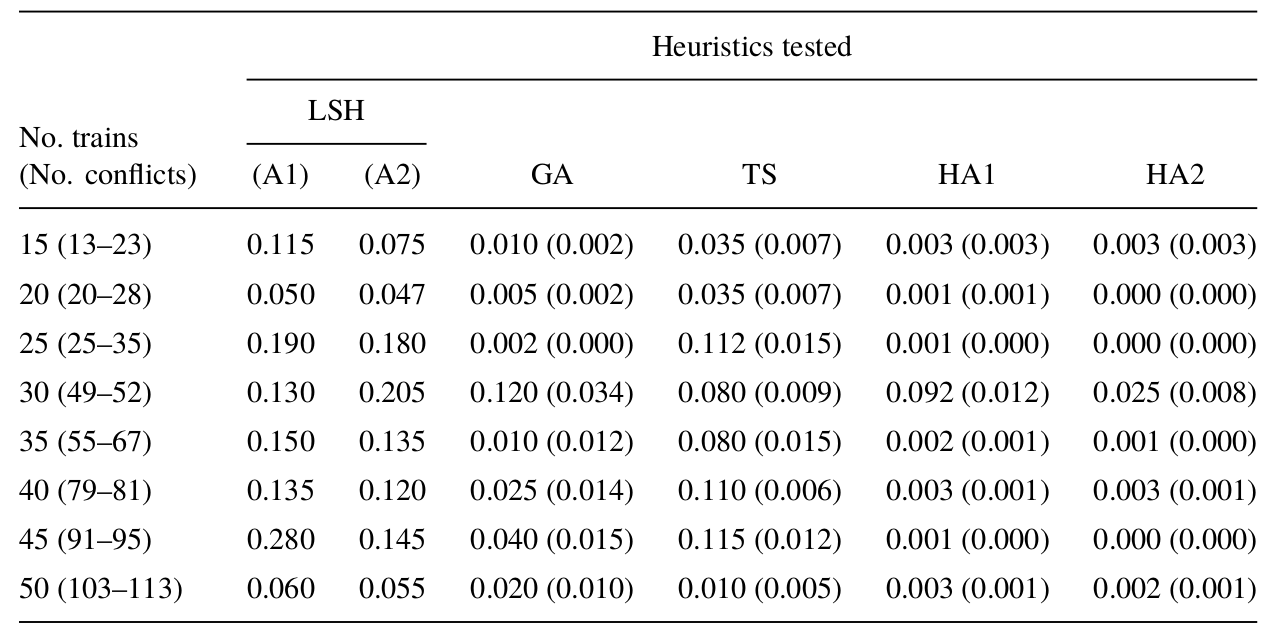
\includegraphics[width=9cm]{rescomp}
	\caption{Comparación de resultados de Heurísticas (Fuente \cite{Higgins})}
	\label{fig:rescomp}
	\end{figure}
	Por otro lado en la Figura \ref{fig:timecomp} se hace una comparación de la capacidad de mejora de la solución, versus los tiempos de procesamiento para cada heurística (se agrega \textit{Branch and Bound} que fué el método para computar la solución óptima). Se puede apreciar que GA, HA1 y HA2 no son capaces de determinar soluciones antes de los $35$ segundos, esto pues primero deben computar la población inicial. Sin embargo luego de computada esta, la razon de convergencia de HA1 y HA2 es superior a la del resto. Por otro lado, se nota que TS y LSH convergen rápido en un inicio, pero luego se estancan. Se termina concluyendo que los algoritmos híbridos son los más viables, y con el mejor desepeño general.

	Otra variante del problema, la constituyen el \textit{Train Rescheduling Problem} en el cual se deben resolver conflictos en tiempo real. Esta es una situación común, en la cual debido a imprevistos (accidentes, retrasos, etc) la planificación prevista debe ser modificada, para poder satisfacer las llegadas/salidas con la menor variación posible. La dificultad se encuentra en realizar una re-planificación aceptable, en el menor tiempo posible. En el trabajo realizado por Norio et al. \cite{Norio}, se propone un modelo de \textit{rescheduling} que intenta minimizar la insatisfacción de la gente. El algoritmo propuesto combina \textit{Program Evaluation and Preview Technique} con el método de \textit{Simulated Annealing}. De modo similar D'Ariano et al. \cite{DAriano} afrontan el mismo problema, pero útlizando el método de \textit{Branch and Bound} (BB). Debido a las restricciones de tiempo, el proceso de BB es acelerado ocupando \textit{reglas de implicación estáticas}, que explotan las propiedades de las soluciones factibles. Las pruebas muestran que el método propuesto es capáz de computar soluciones óptimas (o cercanas) en tiempos pequeños.

	Un problema con mayor parecido al que se trata aquí, es el \textit{Multi Objetive Train Scheduling Prolem}. El problema tratado por Ghoseiri et al \cite{Ghoseiri} se asemeja bastante al de este estudio, en cuanto a las estructura que considera: Una red de pistas compuestas por pistas simples, múltiples pistas, múltiples plataformas (con capacidad de movilidad entre ellas), y múltiples plataformas con distinta capacidad. Sin embargo los objetivos que se plantea son: 1) Minimizar la utilización de combustible (medida de eficiencia que aumenta satisfacción de compañia) y 2) minimizar el tiempo de los pasajeros (medida de eficacia que aumenta la satisfacción de pasajeros). Una formulación diferente la plantea Li et al. \cite{Li}, considerando en sus objetivos: 1) Minimizar la cantidad de energía utilizada, 2) Minimzar los costos de emisiones de carbón, y 3) Minimizar el tiempo de los pasajeros. Debido a sus objetivos, sus autores llaman al modelo \textit{green train scheduling problem}.   

	\begin{figure}[htpb!]
	\centering
	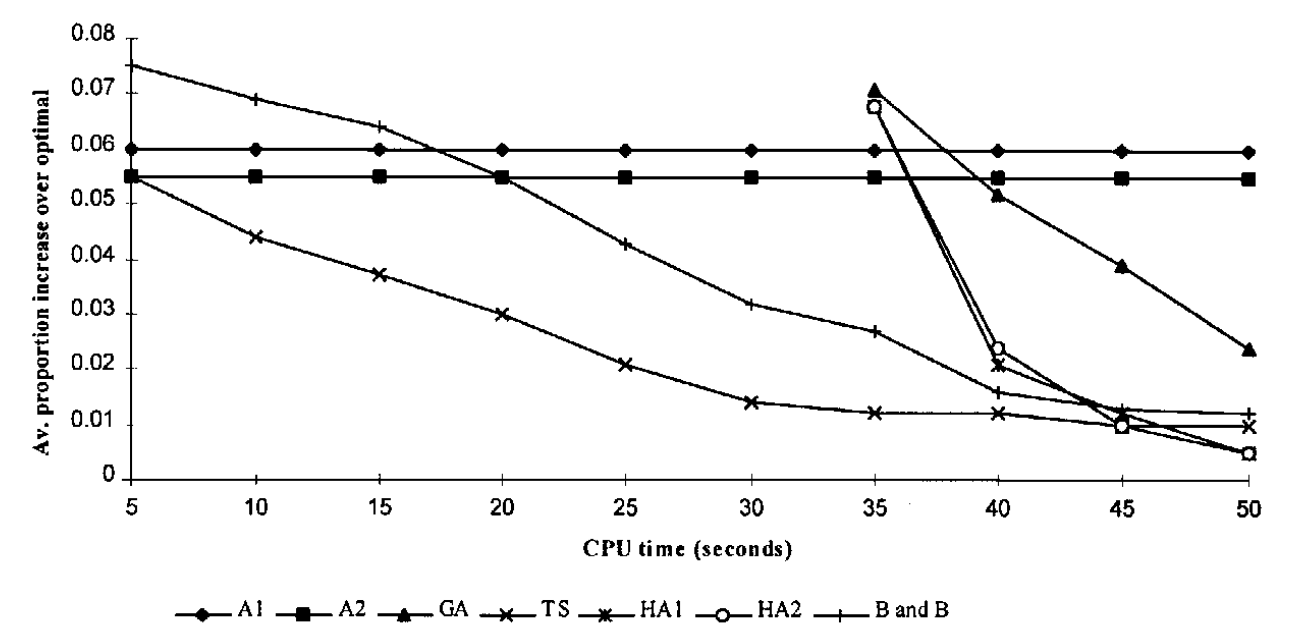
\includegraphics[width=9cm]{timecomp}
	\caption{Comparación de convergencia versus tiempo de ejecución de Heurísticas (Fuente \cite{Higgins})}
	\label{fig:timecomp}
	\end{figure}





\end{description}

\section{Modelo Matemático} \label{model}


\section{Conclusiones} \label{conclutions}


\section{Bibliografía}

\bibliographystyle{plain}
\bibliography{referencias}

\end{document} 